\textbf{Ejemplo 9}\\
Hallar el valor presente con un interés del 2% período año vencido de la siguiente gráfica:\\ \\
%\newpage %USAR SOLO SI EL SOLUCIÓN QUEDA SOLO Y ES NECESARIO BAJARLO A LA SIGUIENTE PAGINA
\textbf{Solución.}\\
%La tabla ira centrada
\begin{center}
 \renewcommand{\arraystretch}{1.5}% Margenes de las celdas
 %Creación de la cuadricula de 3 columnas
 \begin{longtable}[H]{|p{0.5\linewidth}|p{0.5\linewidth}|}
  \hline
  \multicolumn{2}{|c|}{\cellcolor[HTML]{FFB183}\textbf{1. Declaración de variables}}                                                                                                                                  \\ \hline
  $R = 800.000 COP$                                                                                        & $i = 2\% \hspace{1mm} pav$                                                                                \\
  $L = 40\%$                                                                                            & $VP =  ?COP $                                                                                                  \\
  $n=6 \hspace{1mm} pav$                                                                                                                                                                                              \\ \hline
  \multicolumn{1}{|c|}{\cellcolor[HTML]{FFB183}\textbf{2. Diagrama de flujo de caja}}                   & \multicolumn{1}{|c|}{\cellcolor[HTML]{FFB183}\textbf{3. Tabla flujo de caja}}                               \\ \hline
  \multicolumn{1}{|c|}{ 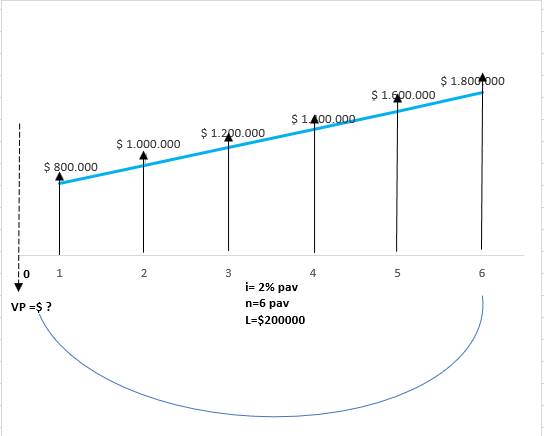
\includegraphics[trim=-5 -5 -5 -5 ,width=0.5\columnwidth]{9/ejemplo9.png}} & \multicolumn{1}{|c|}{ 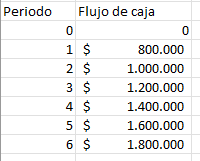
\includegraphics[trim=-5 -5 -5 -5 ,width=0.5\columnwidth]{9/Tabla de flujo Ejem 9.png}} \\ \hline
  \multicolumn{2}{|c|}{\cellcolor[HTML]{FFB183}\textbf{4. Aplicación de funciones}}                                                                                                                                   \\ \hline
  \multicolumn{2}{|p{\columnwidth}|}{Se aplicará la función VNA de la siguiente forma: \newline
  =+VNA (B4; E8:E13) con referencia en la hoja de Excel usada para el ejercicio}                                                                                                                                      \\
  \multicolumn{2}{|l|}{VNA (Valor neto actual): Devuelve el valor presente neto para una inversión}                                                                                                                              \\
  \multicolumn{2}{|c|}{ 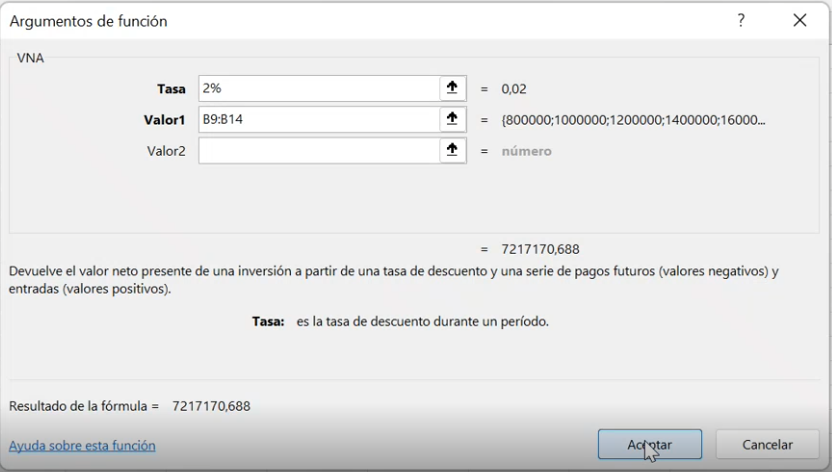
\includegraphics[trim=-5 -5 -5 -5 ,width=0.8\columnwidth]{9/Ejem9.PNG}}                                                                                                                       \\ \hline
  \multicolumn{2}{|c|}{\cellcolor[HTML]{FFB183}\textbf{4. Desarrollo en Excel}}                                                                                                                                       \\ \hline
  \multicolumn{2}{|l|}{Se aplicará la función VNA de la siguiente forma:}                                                                                                                                              \\
  \multicolumn{2}{|l|}{=VNA (0,02; B9;B14) con referencia en la hoja de Excel usada para el ejercicio.}                                                                                                                 \\ \hline
  \multicolumn{2}{|c|}{\cellcolor[HTML]{FFB183}\textbf{5. Gráfico}}                                                                                                                                                   \\ \hline
  \multicolumn{2}{|c|}{ 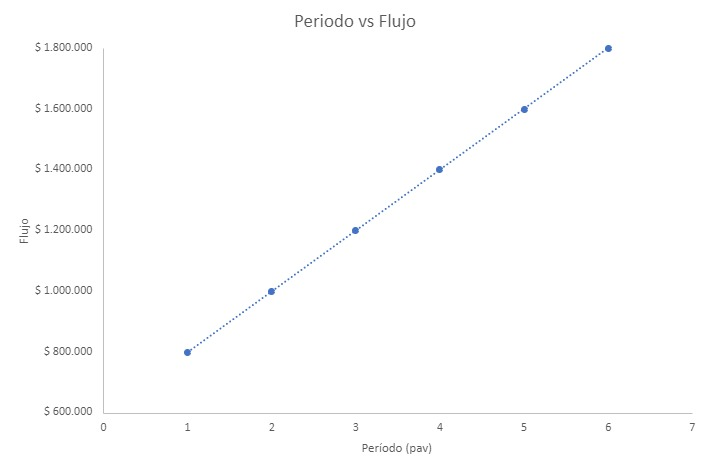
\includegraphics[trim=-5 -5 -5 -5 ,width=0.6\columnwidth]{9/grafico9.png}}                                                                                                                     \\ \hline
  \multicolumn{2}{|c|}{\cellcolor[HTML]{FFB183}\textbf{6. Resultado}}                                                                                                                                                 \\ \hline
  \multicolumn{2}{|c|}{El valor presente es  7.217.170 COP,15}                                                                                                                                                               \\ \hline
 \end{longtable}
 %\newline \newline %USARLO SI CREES QUE ES NECESARIO
\end{center}